\documentclass[../main.tex]{subfiles}

\begin{document}
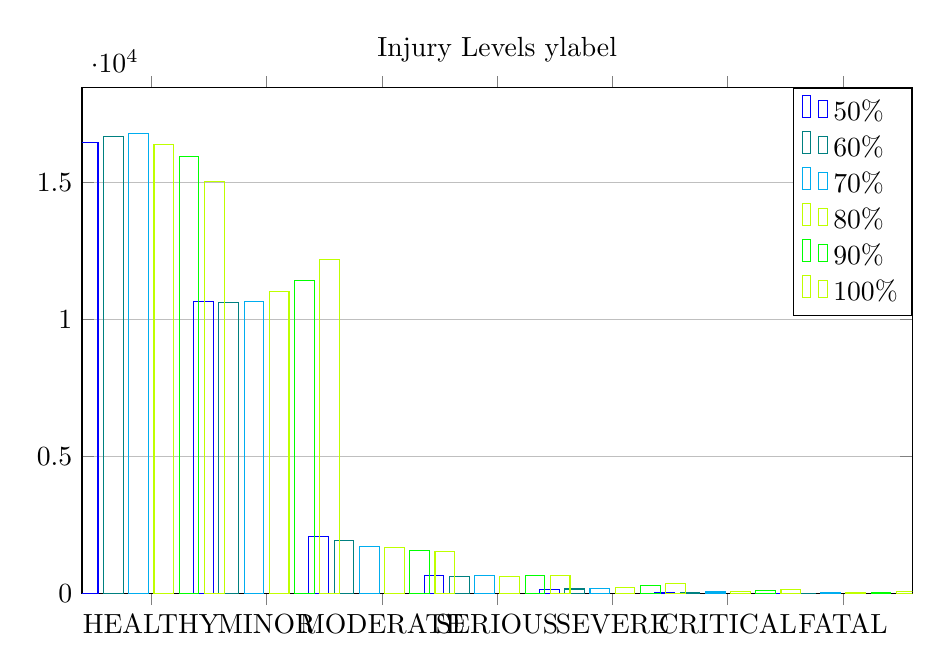
\begin{tikzpicture}
\begin{axis}[
ybar, % style of the histogram: clustered columns
width=\textwidth, % width of the plot
height=8cm, % height of the plot
title={Injury Levels}
ylabel={Amount}, % label for the y-axis
symbolic x coords={HEALTHY,MINOR,MODERATE,SERIOUS,	SEVERE,CRITICAL,FATAL}, % labels for the x-ticks
xtick=data, % position the x-ticks at the data points
ymin=0, % minimum value of the y-axis
legend style={at={(1,1)}, anchor=north east}, % position of the legend
legend cell align=left, % alignment of the legend cells
ymajorgrids=true, % display major grids
bar width=0.25cm % width of the bars
]
\addplot[color=blue] coordinates{(HEALTHY,16459)(MINOR,10648)(MODERATE,2090)(SERIOUS,659)(SEVERE,128)(CRITICAL,12)(FATAL,4)
}; % plot of the first histogram
\addplot[color=teal] coordinates{(HEALTHY,16679)(MINOR,10612)(MODERATE,1914)(SERIOUS,616)(SEVERE,154)(CRITICAL,22)(FATAL,3)
}; % plot of the second histogram
\addplot[color=cyan] coordinates{(HEALTHY,16787)(MINOR,10648)(MODERATE,1698)(SERIOUS,641)(SEVERE,168)(CRITICAL,46)(FATAL,12)
}; % plot of the third histogram
\addplot[color=lime] coordinates{(HEALTHY,16404)(MINOR,11031)(MODERATE,1661)(SERIOUS,606)(SEVERE,212)(CRITICAL,63)(FATAL,23)
}; % plot of the fourth histogram
\addplot[color=green] coordinates{(HEALTHY,15966)(MINOR,11413)(MODERATE,1572)(SERIOUS,637)(SEVERE,274)(CRITICAL,98)(FATAL,40)
}; % plot of the fifth histogram
\addplot[color=lime] coordinates{(HEALTHY,15051)(MINOR,12203)(MODERATE,1511)(SERIOUS,663)(SEVERE,347)(CRITICAL,149)(FATAL,76)
}; % plot of the first histogram
\legend{50\%, 60\%, 70\%, 80\%, 90\%, 100\%} % legend of the plot
\end{axis}
\end{tikzpicture}
\end{document}